\newpage
\appendix
\newpage
\etocdepthtag.toc{mtappendix}
\etocsettagdepth{mtchapter}{none}
\etocsettagdepth{mtappendix}{subsection}
\etoctocstyle{1}{Appendix - Contents}
\tableofcontents
\newpage


\chapter{First Appendix}


\chapter{Second Appendix}
This part aims to give background information about this thesis in the field of filtering methods on nerve tracts using data collected by diffusion MRI. 

% \renewcommand{\thesection}{\Alph{section}}
% \renewcommand{\thesubsection}{\Alph{subsection}}

\section{Diffusion Magnetic Resonance Imaging}
\label{sec:dmri}

Diffusion magnetic resonance imaging (dMRI) has led to discoveries of microstructure and connectivity in human brain.
It is the only non-invasive way to 
systematically map white matter tracts in human brain.
dMRI exploits the natural movement of water molecules 
which exists in micro brain tissues. 
This natural movement, as known as Brownian motion, 
is regarded as random motion of molecules. 

The random displacements of molecules 
resulting from thermal agitation (Brownian motion) 
obey a statistical law established by Einstein in 1905 \cite*{lebihanLookingFunctionalArchitecture2003}.
Diffusion refers to this phenomenon.
And distance of movements could be described by diffusion coefficient.
If molecules are in a free space, the displacements will obey Gaussian distribution
during a given time period. This kind of diffusion can be viewed as isotropic diffusion.

However, not all the molecules are free inside brain. As it shows in Fig. \ref{fig:brownian},
some of them are constraint inside cells, so their displacements are limited by the size of cells. 
Some other molecules are in a narrow space with obstacles, which only allows molecules
to move along a pathway. Displacements are constraint under this situation.
Molecules are far from "free", so the displacements will not fit in standard Gaussian distribution anymore.
This kind of restricted diffusion is known as anisotropic diffusion.
These phenomena can be captured by diffusion tensor with dMRI, which indirectly reveal the microstructure of brain tissue.
This ability of dMRI is particularly effective for studying the connectivity of the brain,
as it permits to noninvasively estimate the major neuronal pathways in the white matter (WM) 
by means of the so called tractography (also known as fiber-tracking) \cite*{daducciCOMMITConvexOptimization2015}.

\begin{figure}[ht]
    \centering
    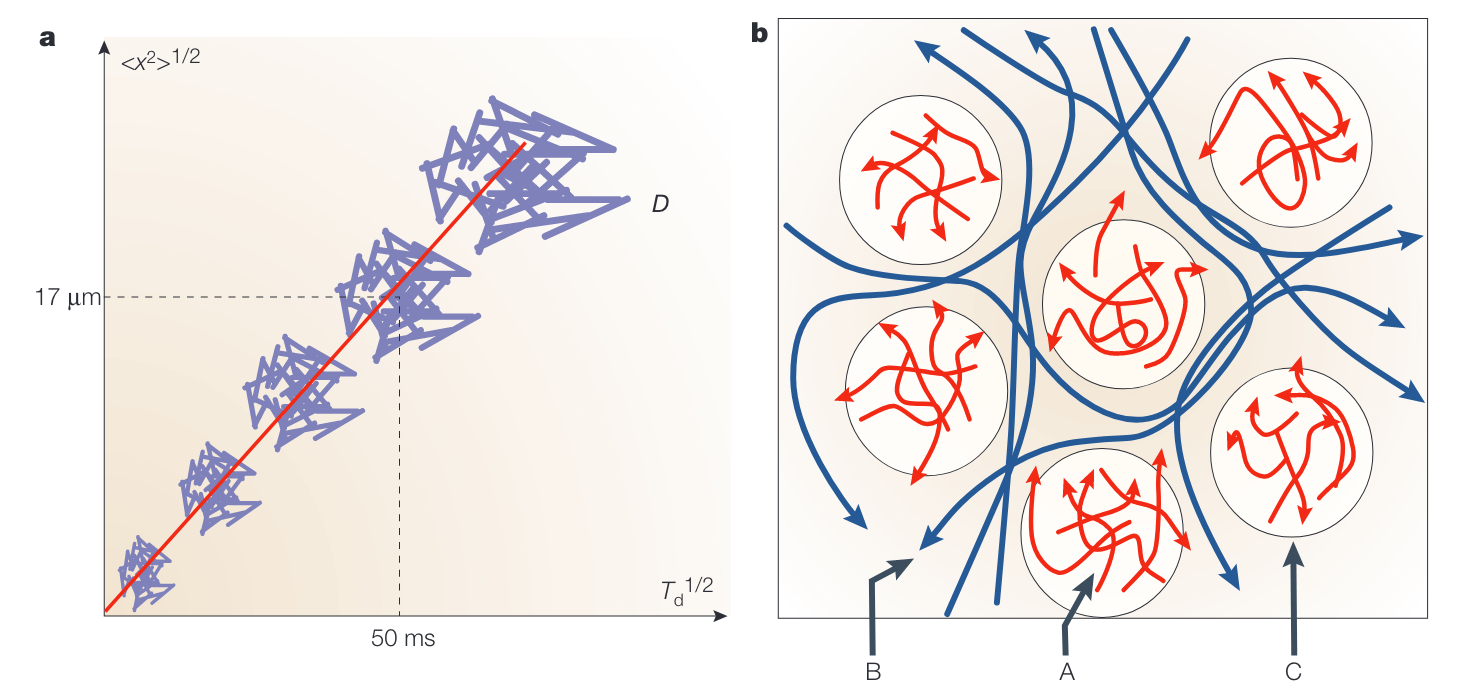
\includegraphics[width= 12cm]{figures/brownian_motion.png}
        \caption{Fig.\textbf{a} shows the relationship among diffusion time, diffusion coefficient and displacement variance.
        ${T_d}$ is the time for molecules to diffuse. $D$ is diffusion coefficient, 
        and <${x^2}$> is the variance of the molecular displacement along that dimension. 
        For water at brain temperature, $68\%$ of molecules have moved within a sphere of $17 \mu s$ diameter in $50 ms$.
        Fig.\textbf{b} mimics biological tissues. Displacements could be constraint in a closed space (A).
        Diffusion might also be hindered by obstacles that result in tortuous pathways (B).
        Exchange between compartments also slows down molecular displacements (C) \cite*{lebihanLookingFunctionalArchitecture2003}.
        }
    \label{fig:brownian}
\end{figure}


\section{Tractography}
\subsection{Diffusion Modeling}

Diffusion data from dMRI will be used to estimate fiber orientations of each voxel. 
This section would introduce some prominent methods and models in this field.

First, standard tensor model introduced by Basser \cite*{Qof40e4TmpElsevier} is the basic model to estimate orientations.
Diffusion tensor in 3D space can be mathematically modeled by a 3 x 3 matrix, which can be written as below. \ref*{tensor_matrix} 
It is a symmetrical, positive tensor consisting of 6 unique parameters. 
Inside $D$, diagonal elements represent diffusion in $x$, $y$ and $z$ coordinates, 
and off-diagonal elements represent correlation of diffusion in two coordinates. 
Diffusion tensor is symmetrical, so it indicates $D_{ij}$ = $D_{ji}$.
Six parameters are enough to build 3 x 3 tensor matrix. 
\begin{gather}\label{tensor_matrix}
    D = 
    \begin{pmatrix}
        D_{11} & D_{12} & D_{13} \\
        D_{21} & D_{22} & D_{23} \\
        D_{31} & D_{32} & D_{33} 
    \end{pmatrix}
\end{gather}

In figure \ref*{fig:DTI}, diffusion tensor imaging(DTI) shows isotropic tensor anisotropic tensor in 
both free space and constraint space. 
$\lambda 1$, $\lambda 2$ and $\lambda 3$ in the tensor model are eigenvalues of diffusion matrix.
Besides, the matrix has three eigenvectors as well. With eigenvalues and eigenvector, the length of diffusion 
and the coordinates of diffusion tensor can be interpreted.

\begin{figure}[ht]
    \centering
    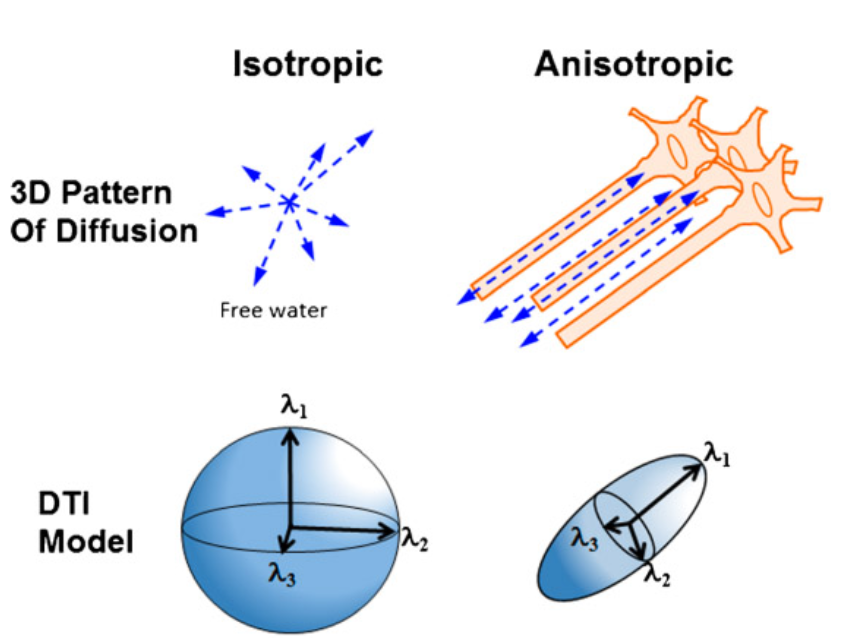
\includegraphics[width= 10cm]{figures/DTI.png}
        \caption{An example showing 3D pattern of diffusion in both free space and constraint space. 
        Second row shows diffusion tensor imaging(DTI) of the according tensor model. 
        $\lambda 1$, $\lambda 2$ and $\lambda 3$ in the tensor model are eigenvalues of diffusion matrix.}
    \label{fig:DTI}
\end{figure}

One major flaw of this model is the inability to represent multiple fiber orientations in a voxel, which can occur due to fiber kissing or crossing \cite*{tournierDirectEstimationFiber2004}.
Besides, there are more pre-defined models including two-tensor model \cite*[]{qaziResolvingCrossingsCorticospinal2009}, ball-and-sticks model \cite*[]{behrensCharacterizationPropagationUncertainty2003}
and neurite orientation dispersion and density imaging (NODDI) model \cite*[]{zhangNODDIPracticalVivo2012}. 
The advantages of these models is that pre-defined patterns in estimating orientations require fewer diffusion sampling directions from dMRI data. 
But when meeting more complex cases such as pathologic data, the results from pre-defined models can't be ensured.

Different from using models, some methods compute the orientational distribution of a voxel. 
Orientation Distribution Functions (ODFs) are the histograms of distribution of diffusion at different dimension. 
Peak values from ODFs can be chosen as orientations during fiber tracking. Methods exploit distribution are flexible with complex condition.
In figure \ref*{fig:odf}, it shows an example of ODF from a voxel computing from samples of multiple directions in dMRI acquisition.

\begin{figure}[ht]
    \centering
    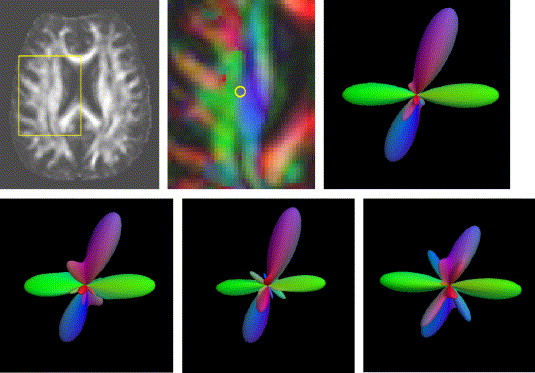
\includegraphics[width= 12cm]{figures/odf.jpg}
        \caption{Fiber ODFs reconstructed from the in vivo data for a voxel.
          Top left: an axial fractional anisotropy(FA) map just below the centrum semiovale. 
          Top middle: a magnified section of the FA map, colored according to the anatomic direction of the major eigenvector of the diffusion tensor 
          (red: left–right, green: anterior–posterior, blue: inferior–superior). 
          Top right: the fiber ODF reconstructed from the highlighted voxel, 
          displayed as a sagittal projection to highlight the presence of the two distinct fiber orientations. 
          Bottom row: fiber ODFs for the same voxel reconstructed using each of the individual 60-direction data sets from data acquisition.
          Note that any negative lobes in the fiber ODF have been discarded. \cite*[]{tournierDirectEstimationFiber2004}
        }
    \label{fig:odf}
\end{figure}

Two types modeling methods mentioned above can be viewed as model-based method and model-free method. 
Spherical deconvolution methods combine both of them. These methods estimate the fiber orientation distribution directly from high angular resolution diffusion-weighted MR data without prior assumptions \cite*[]{tournierDirectEstimationFiber2004}.
On the one hand, these methods also computes ODFs as model-free methods. 

Different from the other two methods, the prior assumption of spherical deconvolution
is that all white matter fiber bundles in the brain share identical diffusion characteristics,
thus implicitly assigning any differences in diffusion anisotropy to partial volume effects \cite*[]{tournierDirectEstimationFiber2004}.
To be specific, the diffusion model in spherical deconvolution comes from selected white matter.
Kernels extracted from diffusion model are called \textit{response functions} and are used to convolve with ODFs.
The results are called fiber orientation distribution (FOD).
Some research indicates that FOD tractography has a better resolving power than DTI and diffusion ODF methods, making it ideal for delineating fibers crossing at a sharp angle \cite*[]{yehTractographyMethodsFindings2021}.
Moreover, all these methods are rather recent, so more studies and validations are needed.

\subsection{Fiber Tracking Methods}

The fiber tracking strategies can be mainly divided into deterministic, probabilistic, and global geometric techniques \cite*[]{ozarslanAnisotropyFieldsScales2021}.
In this paper, we would mainly introduce streamline tracking, a deterministic technique, that is most commonly used algorithm for tractography.

With local data available in the neighborhood of each voxel, fiber tracking can be viewed as solving an \textit{ordinary differential equation} (ODE), 
and the targeted track trajectory is the unknown function to be estimated \cite*{daducciCOMMITConvexOptimization2015}\cite*{yehTractographyMethodsFindings2021}.
The goal of the first-order ODE problem is to numerically estimate an unknown function using both its first derivatives and an initial value of the function \cite*[]{yehTractographyMethodsFindings2021}.
In streamline tracking, the initial value would be the starting point of the trajectory, while the diffusion field is used to interpret derivatives.
Usually the initial values are defined manually. For example, a deterministic algorithms Fiber Assigned by Continuous Tracking (FACT), 
a starting point in gray matter is chosen to be along the biggest main eigenvector of the adjacent voxels. 
% \cite{}
This propagating process from starting point is repeated by integrating in diffusion field at each position until any of termination criteria are met. These criteria include
meeting the boundary of masks and maximum turning angle. 

In figure \ref*{fig:tracking}, the first scenario shows how to use Euler method in calculating fiber trajectory. 
This method also starts with pre-defined points, as known as seeds, and propagates in two opposite directions. At each voxel, the spatial 
information of next voxel is determined by the present voxel and its derivative, 
which can be viewed as $f(t_{i+1}) = f(t_{i}) + f'(t_{i})\Delta s$. And $\Delta s$ here is the step size in propagation.
After propagation on every given seed, all streamlines are finally generated.
The set of obtained streamlines is usually referred to as a tractogram

\begin{figure}[ht]
    \centering
    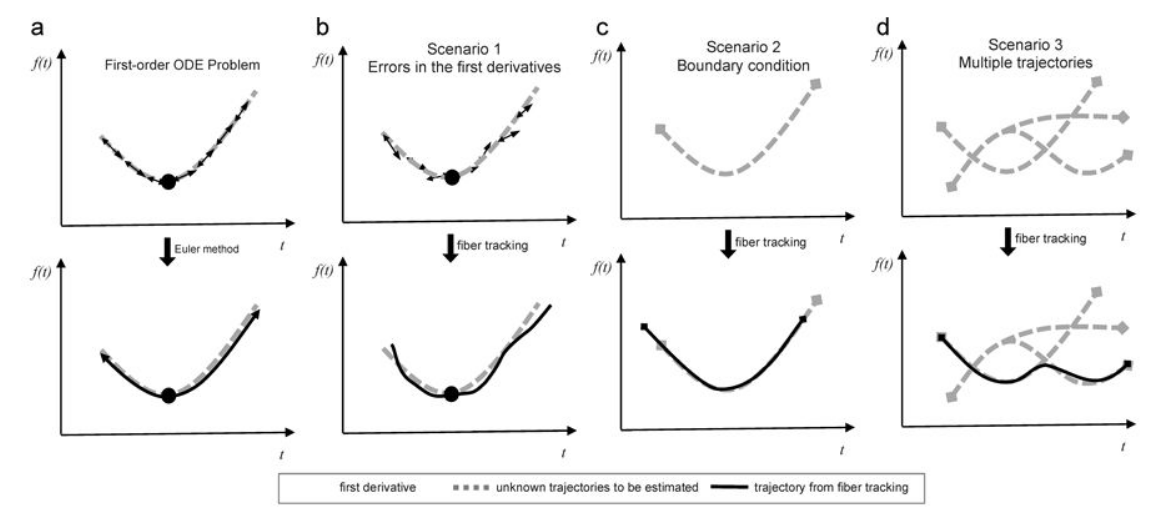
\includegraphics[width= 13cm]{figures/tracking.png}
        \caption{Fiber tracking involves a numerical procedure to solve a first-order ordinary differential equation (ODE) whose parameters are specified by a starting location (i.e., the seeding point, black circle) 
        and by the first derivative of a function (i.e., the resolved fiber orientation, arrows) at each voxel. 
        The trajectory can then be calculated using the Euler method. 
        However, the conventional ODE problem only considers numerical error due to finite step size and does not consider other error scenarios in fiber tracking. 
        The first scenario that raises challenges for standard fiber tracking involves errors in the estimation of first derivatives, 
        which can cause substantial deviation of trajectories from their ground truth. 
        The second challenging scenario involves the boundary condition. Specifically, white matter tracts have termination locations, and fiber tracking may terminate at the wrong location, 
        leading to a premature termination or an overshoot.
        The third challenging scenario involves the coexistence of multiple trajectories at the same voxel location. 
        Inappropriately connecting unrelated trajectories may lead to incorrect streamline routing and spurious tracks. \cite*[]{yehTractographyMethodsFindings2021}
        }
    \label{fig:tracking}
\end{figure}

However, fiber tracking methods suffer from errors. As it shows in the scenario 1 in figure \ref*{fig:tracking},
sometimes local angles can't match properly, which may due to limitation in diffusion modeling or artifact in data acquisition.
Scenario 2 shows the problem with termination criteria. In scenario 3, when multiple trajectories locate in the same space,
it adds difficulty to fiber tracking. Sometimes the tracking method chooses a wrong direction and connects to another nearby fiber.
It is common error when the voxel has complex diffusion.

\subsection{Tractogram Filtering}

Despite the advances in tractography methods, the anatomical accuracy of tractography has not dramatically improved in recent years \cite*[]{schillingLimitsAnatomicalAccuracy2019}.
First, tractography techniques are mainly based on mathematical computation. Not many anatomical requisites have been applied
to it. And we have discussed some limitations in both diffusion modeling and tractography techniques, which remain uncertainty.
Moreover, in the analysis of brain connectivity realized by dMRI, high specificity has been a challenge to tractography.
This refers to the false positives in tractograms.
Several recent studies have unveiled that state-of-the-art methods to construct tractograms suffer both from false positives (FP), 
i.e., streamlines that are not related to anatomical structures \cite*[]{maier-heinChallengeMappingHuman2017}.
The false positive streamlines create bias in any connectivity analysis since non-existent structures are mixed with real ones \cite*[]{gleichgerrchtDeepLearningApplied2018}. 
To reduce the influence of this bias, some methods are used to improve the tractogram quality. 
This section briefly summaries four main methods in tractogram filtering:
\textit{explainability of the diffusion signal, inclusion and exclusion of regions of interest, streamline geometry and shape and streamline similarity and clustering.} 


\subsubsection{Explainability of the diffusion signal}

A tractogram is based on the diffusion signal from dMRI. 
Therefore, synthetic dMRI generated back from a tractogram should be similar to raw data.
The idea of this method is to find a subset of the streamlines that best describes the input dMRI data. 
This method requires dMRI data and a whole tractogram as inputs.

The Convex Optimization Modeling for Microstructure Informed Tractography (COMMIT) \cite*[]{daducciCOMMITConvexOptimization2015} and LiFE \cite*[]{pestilliEvaluationStatisticalInference2014}, 
describe this filtering method in a mathematical way. 
In equation \ref*{explaindiffusion}, $y$ is the vector with the input diffusion signals. 
$A(T)$ is the formula to synthesize the diffusion data from the streamlines of tractogram $T$, 
while $x$ is the vector with weight for each streamline. And $\eta$ is the acquisition noise. 
Since the $x$ that represents the weights of streamlines will not be negative, 
it is possible to find a minimum for $\eta$. 

\begin{gather}\label{explaindiffusion}  
    y = A(T)x + \eta\\
    \underset{x>=0}{argmin}||A(T)x-y||_{2}^{2}
\end{gather}



SIFT \cite*{smithSIFTSphericaldeconvolutionInformed2013} and SIFT2 \cite*{smithSIFT2EnablingDense2015} share the same idea of explainability,
but their purpose is not to synthesize raw dMRI data with the best combination of streamlines. 
Instead, they focus on removing the less relevant streamlines for better fitting raw data.
Specificlly, the algorithms remove streamlines iteratively to find the minimal sets of streamlines.
However, the removed streamlines won't come back to the results, which means this method can run into local minima.
Another difference of SIFT from the other methods is that it only generate binary labels of streamlines.


Based on this method, a common problem with some mentioned tools is inconsistency in results. 
In practice, results on the same tractogram from either SIFT or COMMIT
sometimes won't be consistent from multiple runtime. 
Same for the same streamline, these tools can't be sure of having the same labels or weight values every time.
The size of tractograms and the length of streamlines can be bias factors to this type of method.

The main purpose of this report is to improve plausibility of the results from COMMIT, 
as well as analyze the impact from multiple biases.


\subsubsection{Inclusion and exclusion of regions of interest}
This method respects the anatomy of the brain by using segmentation masks to filter false positive streamlines. 
To achieve an anatomically correct segmentation, registration to standard atlas is required. 
Streamlines totally outside masks or against anatomical atlas will be filtered. 
The intrinsic problem with this method is about inaccurate registration.
For example, shape of neural fibers changes when a tumour continuously growing inside the brain. 
Using these methods to register dMRI data of a pathologic brain to a standard healthy atlas is not reasonable.
Moreover, registration of brain brings uncertainty as well.


\subsubsection{Streamline geometry and shape}

This method exploits geometrical properties of streamlines.
Shape features of streamlines include the maximum local curvature, the maximum and minimum length of streamlines and so on. 
Some characteristics not existing in real brain should be avoided, such as an unrealistic loop of streamlines. 

Deep learning methods have taken geometry of streamlines as criteria, such as TRAFIC \cite*{lamTRAFICFiberTract2018}. 
It trains a neural network with features such as distances to five landmarks, curvature and torsion per tract as features for filtering \cite*{lamTRAFICFiberTract2018}.

\subsubsection{Streamline similarity and clustering}

The number of streamlines can easily reach 10 million before analysis. 
This method helps cluster streamlines in bundles before analysis. 
From the view of analysis, small bundles that contribute little to the connectivity analysis can be filtered. 
So the only requirement for using standard clustering algorithms for streamline clustering 
is to define a distance metric between streamlines \cite*[]{ozarslanAnisotropyFieldsScales2021}.
The method seems to be very straightforward, but it's not easy to find the best distance for all streamlines.


\section{Deep Learning Methods}
\subsection{Multilayer Perceptron (MLP)}

\section{Structural Connectivity Networks}

% \subsection{Brain connectivity}
% As we know, brain is the main processor of human. 
% It's a complex organ in charges of sense, motor motion, emotion, vision, breathing and
% every process happening to human body.
% Inside brain, neuron is the key unit that support brain to execute all the processes.
% A neuron has three main parts: dendrites, an axon, and a cell body (soma).

\subsection{Brain Connectivity Creation Pipeline}

